\section{Speed of Polarization}
\lecture{25 Mar.}

Referring back to Theorem \ref{thm:w1_polar_speed}, where we established the speed at which BECs polarize. Now let us delve deeper into the analysis and show some of the missing details while connecting with what we have learned. The papers ``Unified Scaling of Polar Codes: Error Exponent, Scaling Exponent, Moderate Deviations, and Error Floors'' \cite{Unified_Scaling_of_Polar_Codes} and ``Sub-4.7 Scaling Exponent of Polar Codes'' \cite{Sub_4_7_Scaling_Exponent} provide more recent advances in finding the scaling exponent and its relationship with other coding theoretical parameters.

Let us assume that there exists a special concave function $f(x)$ (an approximation would be $\approx[x(1-x)]^{2/3}$, with another commonly used exponent is 0.7). By concavity, we have that
\begin{align*}
    &f(x^2) + f(2x-x^2) \le 2f(x) \\&\Rightarrow f\left(P_e(\mathrm{BEC}(x)^+)\right) + f\left(P_e(\mathrm{BEC}(x)^-)\right) \le 2 f\left(P_e(\mathrm{BEC}(x))\right).
\end{align*}
This is how this special function is linked with BECs. Furthermore, we are interested in the following quotient (see also the figure below) that is between 0 and 1:
\begin{equation}
    \lambda \defeq \sup_{0\le x\le 1} \frac{f(x^2) + f(2x-x^2)}{2f(x)}. \label{eq:w6_polarization_lambda}
\end{equation}

We have already shown that
\begin{equation}
    \frac{1}{2^n}\sum_{s\in\{+,-\}^n}f\left(P_e(\mathrm{BEC}(x)^s)\right) \le \lambda^n f(x).
\end{equation}
Hence as $n\rightarrow\infty$, we have that $f\left(P_e(\mathrm{BEC}(x)^s)\right)$ approaches 0 for all $s$, meaning that $P_e(\mathrm{BEC}(x)^s)=0$ or $1$ for all $s$. This is our characterization of the speed of polarization. 

For all possible convex $f$, which produces the smallest $\lambda$? It is obvious that for $[x(1-x)]^{2/3}$, the $\lambda$ is not optimal. How do we find the optimal $f$? Simply by the power method.

\begin{remark}
    Let us take a small detour into the ``power method'' from linear algebra, which is very similar to the question proposed above.

    Given a matrix $A$, we would like to find the eigenvalue with the largest absolute value, i.e.
    \begin{equation*}
        \abs{\lambda_1} = \max_{\vec{x}} \frac{\norm{Ax}}{\norm{x}},
    \end{equation*}
    where the norm is the Euclidean norm. The maximum is achieved when $\vec{x}=\vec{x}_1$, the eigenvector corresponding to the eigenvalue $\lambda_1$. A useful method in finding $\vec{x}$, and hence $\lambda_1$, is the power method, in which one simply iterates the map
    \begin{equation*}
        \vec{x} \leftarrow \varphi(\vec{x}) = \frac{A\vec{x}}{\norm{\vec{x}}}.
    \end{equation*}
    Then we have $\varphi^n(\vec{x})\rightarrow\vec{x}_1$ as $n\rightarrow\infty$.
\end{remark}

For BECs, let us define the following operator
\begin{equation}
    T_{\mathrm{BEC}}(f) = \frac{f(x^2)+f(2x-x^2)}{2}.
\end{equation}
% Since the erasure probability of BECs under the polarization process is a martingale,
% \begin{equation}
%     \mathbb{E}[f(P_{e,n)}\vert P_{e,0}] = \overbrace{T_{\mathrm{BEC}}\circ T_{\mathrm{BEC}}\circ\cdots\circ T_{\mathrm{BEC}}}^{n\text{ times}}(f).
% \end{equation}
Then \autoref{eq:w6_polarization_lambda} will be equivalent to finding the largest eigenvalue to the eigenvalue problem
\begin{equation}
    T_{\mathrm{BEC}}(f) = \lambda f(x).
\end{equation}
However, we always have the trivial largest eigenvalue of $\lambda=1$ for $f(x)=1$ and $f(x)=x$. Hence, we are to find the largest eigenvalue $\lambda^*$ other than $1$.


By the power method, we define the following iteration scheme:
\begin{equation}
    f \leftarrow \frac{f(x^2) + f(2x-x^2)}{2\sup_{x\in[0,1]}f(x)}. \label{eq:w6_polar_speed_fxn}
\end{equation}
In the end when this iteration converges, the supremum is $\lambda^*=2^{-1/\mu^*}$, the value $\mu^*$ is coined the scaling exponent.

\begin{figure}[H]
    \centering
    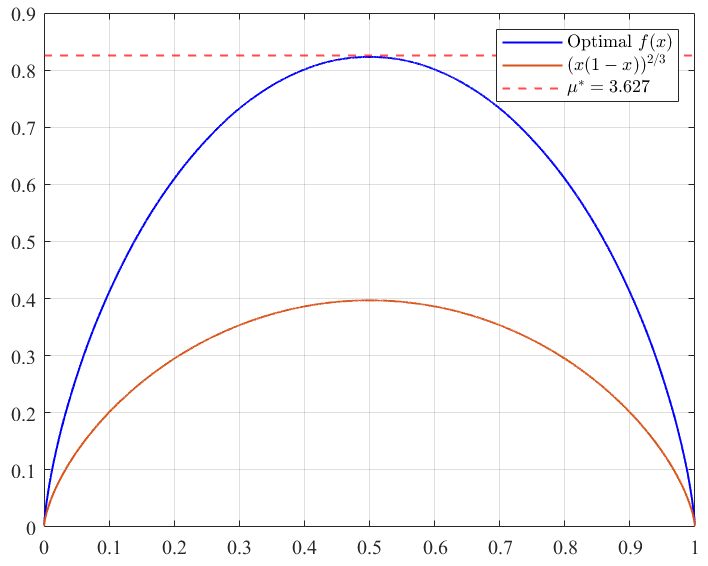
\includegraphics[width=0.6\linewidth]{figures/w6_polarization.png}
    \caption{Eigenfunction to $T_\mathrm{BEC}$.}
    \label{fig:w6_eigfxn}
\end{figure}

Using $(x(1-x))^{2/3}$ as the initial condition, the algorithm quickly converges to \autoref{fig:w6_eigfxn}, with the optimal scaling exponent equal to $\mu^*=3.627$.

\begin{remark}
    Why does \autoref{eq:w6_polar_speed_fxn} converge?
\end{remark}

Previously in \autoref{eq:w3_martingale_conv}, we considered $M_n$ as the polarization process of $\mathrm{BEC}(x)$, and by arguments of martingale convergence theorem, we have seen that
\begin{equation*}
    \mathrm{Pr}\{M_n\in(\varepsilon,1-\varepsilon)\} < \delta
\end{equation*}
is a constant bound on the converging probability. We can do better than this by introducing the optimal $f$ (optimal as in the arguments above) to have
\begin{align*}
    \mathrm{Pr}\{M_n\in(\varepsilon,1-\varepsilon)\} &= \mathrm{Pr}\{f(M_n) > f(\varepsilon)\} \\
    &\le \frac{\mathbb{E}[f(M_n)]}{f(\varepsilon)} \\
    &\approx 2^{-\frac{n}{3.627}} f(M_0) / f(\varepsilon).
\end{align*}
We can see that the speed of polarization is exponentially fast.

\begin{remark}
    Besides plugging in $x$ as the error probability, we have also learned that the Bhattacharyya parameter $Z$ as an equivalent description of channel quality! For BECs, the Bhattacharrya parameter $Z_n$ follows the same polarization process as $P_e$, and hence has the same polarization speed. 
    
    However, for more general BMSCs, the Bhattacharyya parameter becomes a supermartingale. By denoting $z=Z(W)$,
    \begin{equation}
        z\sqrt{2-z^2} \le Z(W^-) \le 2z-z^2,
    \end{equation}
    the iteration \autoref{eq:w6_polar_speed_fxn} hence needs to be updated as
    \begin{equation}
        f \leftarrow \sup_{x\sqrt{2-x^2} \le y \le 2x-x^2} \frac{f(x^2)+f(y)}{2\sup_{x\in[0,1]}f(x)}.
    \end{equation}
    In this case, the scaling exponent obtained will be $\mu^*=4.717$, just as described in \autoref{thm:w1_polar_speed}.
\end{remark}

\section{Large Kernel of Polar Code}
Previously in polar code, we have only been consider the $2\times 2$ kernel $\left[\begin{matrix}
    1 & 0 \\ 1 & 1
\end{matrix}\right]$ as proposed by Ar{\i}kan, where each encoding and decoding block has two input and two outputs. However, this can be modified to allow for a larger kernel.

If we consider
\begin{equation*}
    A = \left[\begin{matrix}
        a_{11} & \cdots & a_{\ell1} \\
        \vdots & \ddots & \vdots \\
        a_{1\ell} & \cdots & a_{\ell\ell}
    \end{matrix}\right] \in \mathbb{F}_2^{\ell\times\ell}
\end{equation*}
as our kernel for polar code, then given the input bits $[u_1,\ldots,u_\ell]$, the encoded bits will be $[x_1,\cdots,x_\ell] = [u_1,\ldots,u_\ell] A$. With the encoded bits as channel inputs, the channel outputs will be $[y_1,\cdots,y_\ell]$. The decoder is again operated by maximum likelihood estimation. The $\ell$ polarized channels will be:
\begin{itemize}
    \item $W^{(1)}$ is guessing $u_1$ given $y_1,\ldots,y_\ell$.
    \item $W^{(2)}$ is guessing $u_2$ given $y_1,\ldots,y_\ell$ and $u_1$.
    \item $W^{(3)}$ is guessing $u_3$ given $y_1,\ldots,y_\ell$ and $u_1,u_2$.
    \item $\vdots$
    \item $W^{(\ell)}$ is guessing $u_\ell$ given $y_1,\ldots,y_\ell$ and $u_1,\ldots,u_{\ell-1}$.
\end{itemize}
The matrix $A$ is termed the \textit{generator matrix} of the code. For more details, and also for the definitions of the terms used in the theorem below, please refer to \autoref{sec:w6_algebra}.

\begin{theorem}
    Consider a code with generator matrix $A$ for a BMSC $W$. Let $A_i$ be the $i$th row to $A$, and $\mathcal{C}_i$ as the code generated by $A_{i+1},A_{i+1},\ldots,A_\ell$. We have the following inequality for the Bhattacharyya parameter:
    \begin{equation}
        Z(W^{(i)}) \le \sum_{w\in\mathcal{C}_i} Z(W)^{\abs{w+A_i}}.
    \end{equation}
\end{theorem}
The function $\abs{w}=d_\mathrm{H}(w,0)$ is the Hamming weight of the codeword $w$. The theorem is stated without a proof. But as a sanity check, let us consider the example below.
\begin{example}
    Consider $W=\mathrm{BEC}(x)$, with $Z(W) = x$. Then let the generator matrix of the code be the Ar{\i}kan matrix
    \begin{align*}
        &A = \left[\begin{matrix}
            1 & 0 \\ 1 & 1
        \end{matrix}\right]\in\mathbb{F}_2^{2\times2}, & A_1=[\begin{matrix}
            1 & 0
        \end{matrix}], &&A_2 = [\begin{matrix}
            1 & 1
        \end{matrix}],
    \end{align*}
    with the code generated being
    \begin{align*}
        &\mathcal{C}_1 = \{00,11\}, &\mathcal{C}_2 = \{00\}.
    \end{align*}
    Then we have
    \begin{align*}
        Z(W^{(1)}) = Z(W^-) = 2x-x^2 &\le \sum_{w\in\mathcal{C}_1} x^{\abs{w+A_1}} = 2x, \\
        Z(W^{(2)}) = Z(W^+) = x^2 &= \sum_{w\in\mathcal{C}_2} x^{\abs{w+A_2}} = x^2.
    \end{align*}
    The theorem indeed holds true.
\end{example}
Moreover, consider the uniformly distributed indices $s_1,s_2,\ldots\in\{1,2,\ldots,\ell\}$. We can define a random process $W_{i+1}=(W_i)^{(s_{i+1})}$ with $W_0 = W$. Then the Bhattacharyya parameter $Z_i=Z(W_i)$ is also a random process. However,
\begin{equation*}
    \mathbb{E}[Z_{i+1}\vert Z_i] = \frac{1}{2}(2x) + \frac{1}{2}(x^2) \not\le x,
\end{equation*}
it is no longer a supermartingale, nor a martingale. This is different from \autoref{thm:channel_param_martingale}. Nevertheless, the following result holds true:
\begin{theorem}
    Define $a\wedge b = \min(a,b)$, then
    \begin{equation}
        X_n = (Z_n\wedge\delta)^\varepsilon
    \end{equation}
    is a supermartingale for $\delta$ and $\varepsilon$ small enough.
\end{theorem}
The theorem is stated without a proof.



\section{Polar Code with Joint Source-Channel Coding} 
We have seen that polar code doing source coding. We have also seen that polar code doing channel coding. Now let us see polar code doing both at the same time. The description of this section follows the paper `` Polar Coding without Alphabet Extension for Asymmetric Models'' \cite{Polar_Coding_wo_Alphabet_Extension_for_Asymmetric_Models} by J. Honda and H. Yamamoto.

As a first example, let us consider $W=(X\vert Y)$ as the $Z$ channel with the optimal input distribution that achieves the channel capacity. Define the channel $V=(X\vert\sim)$ that sends nothing. We can define both $W^{\pm\pm\ldots}$ and $V^{\pm\pm\ldots}$, and they will both be polarized: $H(W^s)\approx 0$ or $1$ and $H(V^s)\approx 0$ or $1$ for all $s\in\{+,-\}^n$. There are a total of four possible combinations (see table below), let us analyze their properties.

\begin{table}[H]
    \centering
    \begin{tabular}{|c||c|c|}
        \hline
        \multirow{2}{*}{\diagbox{$H(V^s)$}{$H(W^s)$}} & \multirow{2}{*}{0} & \multirow{2}{*}{1} \\ 
        & & \\
        \hline\hline
        0 & (A) & (B) \\ \hline
        1 & (C) & (D) \\ \hline
    \end{tabular}
    \caption{Classification of bits: A is for source coding. B is impossible. C is for channel coding. And D is the frozen bits.}
\end{table}

\begin{itemize}
    \item (B): One can show that $\mathrm{Pr}\{\text{B}\}=0$, hence this combination is not possible.
    \item (D): $\mathrm{Pr}\{\text{D}\} = H(W_0) = H(W)$.
    \item (C): Since $\mathrm{Pr}\{\text{C}\cup\text{D}\} = H(V_0) = H(X)$, hence $\mathrm{Pr}\{\text{C}\} = H(X)-H(W) = H(X) - H(X\vert Y) = I(W)$. If we let C be the information bits, then we see that it is in fact capacity-achieving. This is the channel coding part.
    \item (A): For $H(V^s)\approx0$, it implies that $u_s$ is almost predictable as it only depend on the previous bits $u_{1:s-1}$. This is the source coding part, to shape the input distribution to be no longer uniformly distributed.
\end{itemize}